\documentclass[tikz,border=2pt]{standalone}

\usepackage{pgfplots}
\pgfplotsset{compat=1.18}

\begin{document}
	
		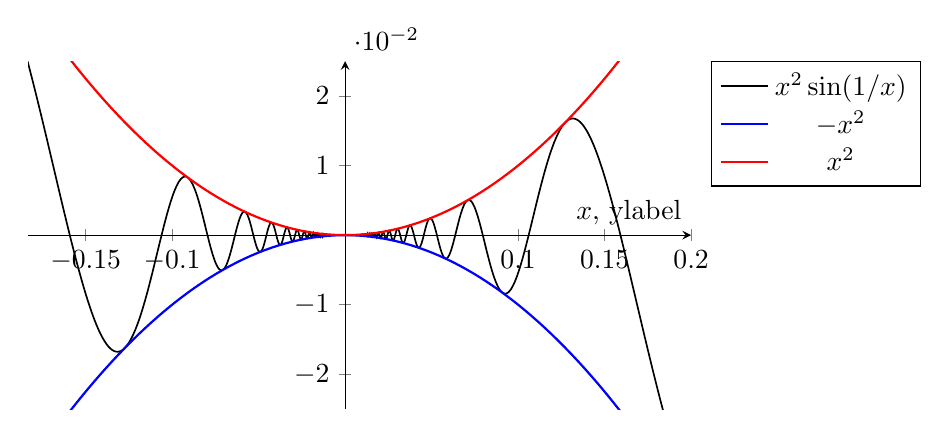
\begin{tikzpicture}
		\begin{axis}[
			axis lines=middle,
			xlabel=$x\text{,}$
			ylabel=$y\text{,}$
			xmin=-0.2, xmax=0.2,
			ymin=-0.025, ymax=0.025,
			xtick={-0.2,-0.15,-0.1,0.1,0.15,0.2},
			ytick={-0.02,-0.01,0,0.01,0.02},
			legend pos=outer north east,
			legend style={cells={align=left}},
			width=10cm,
			height=6cm
			]
			\addplot[
			domain=-0.2:0.2,
			samples=1000,
			color=black,
			line width=0.6pt
			]{x^2*sin(deg(1/x))};
			\addlegendentry{$x^2\sin(1/x)$}
			\addplot[
			domain=-0.2:0.2,
			samples=100,
			color=blue,
			line width=0.8pt
			]{-x^2};
			\addlegendentry{$-x^2$}
			\addplot[
			domain=-0.2:0.2,
			samples=100,
			color=red,
			line width=0.8pt
			]{x^2};
			\addlegendentry{$x^2$}
		\end{axis}
	\end{tikzpicture}
	
\end{document}